% =============================================================================
%  课程作业报告：门控全信息策略梯度（GFPG）
%  编译：在 report/ 目录执行  latexmk -xelatex main.tex  （或 xelatex 两次）
%  所有实验数值来自 generated/*.tex，由 scripts/make_figures.py 从实验产物自动生成。
% =============================================================================
\PassOptionsToPackage{table}{xcolor}
\documentclass[a4paper,zihao=5,linespread=1.38]{ctexart}

\usepackage[a4paper,top=2.5cm,bottom=2.4cm,left=2.4cm,right=2.4cm,
            headheight=15pt,headsep=0.75cm,footskip=1.1cm]{geometry}

% ---------------------------------------------------------------- fonts
\usepackage{amsmath,mathtools}
\usepackage{unicode-math}
\setmainfont{STIXTwoText}[Extension=.otf, UprightFont=*-Regular, BoldFont=*-SemiBold,
                          ItalicFont=*-Italic, BoldItalicFont=*-SemiBoldItalic]
\setsansfont{SourceSansPro}[Extension=.otf, UprightFont=*-Regular, BoldFont=*-Semibold,
                            ItalicFont=*-RegularIt, BoldItalicFont=*-SemiboldIt]
\setmonofont{SourceCodePro}[Extension=.otf, UprightFont=*-Regular, BoldFont=*-Bold, Scale=0.86]
\setmathfont{STIXTwoMath-Regular.otf}
% CJK fonts: modern macOS families when available; ctex's automatic fontset otherwise.
\IfFontExistsTF{Songti SC}{%
  \setCJKmainfont{Songti SC}[BoldFont={Songti SC Bold}, ItalicFont={Kaiti SC}, BoldItalicFont={Kaiti SC Bold}]}{}
\IfFontExistsTF{PingFangSC-Regular}{%
  \setCJKsansfont{PingFangSC-Regular}[BoldFont={PingFangSC-Semibold}]
  \setCJKmonofont{PingFangSC-Regular}}{}
\setlength{\emergencystretch}{2em}

% ---------------------------------------------------------------- packages
\usepackage{graphicx}
\graphicspath{{figures/}}
\usepackage{booktabs,tabularx,multirow,array,makecell}
\newcolumntype{L}{>{\raggedright\arraybackslash}X}
\usepackage{xcolor}
\usepackage[most]{tcolorbox}
\usepackage[ruled,vlined,linesnumbered]{algorithm2e}
\usepackage{tikz}
\usetikzlibrary{arrows.meta,positioning,calc,fit,backgrounds}
\usepackage{fancyhdr}
\usepackage{enumitem}
\usepackage{caption}
\usepackage{float}
\usepackage{xurl}
\usepackage{hyperref}
\usepackage{bookmark}

% ---------------------------------------------------------------- colours
\definecolor{accent}{HTML}{2A78D6}
\definecolor{accentdark}{HTML}{17406D}
\definecolor{accentwash}{HTML}{EEF4FC}
\definecolor{ink}{HTML}{0B0B0B}
\definecolor{ink2}{HTML}{52514E}
\definecolor{muted}{HTML}{898781}
\definecolor{hair}{HTML}{E1E0D9}
\definecolor{warm}{HTML}{EB6834}
\definecolor{warmdark}{HTML}{A8431C}
\definecolor{warmwash}{HTML}{FDF1EB}
\definecolor{rowhighlight}{HTML}{EAF2FC}
\definecolor{good}{HTML}{0B7A0B}

\hypersetup{colorlinks=true, linkcolor=accentdark, citecolor=accent, urlcolor=accent,
            pdftitle={GFPG：门控全信息策略梯度——面向 LLM Harness 受限自我改进的梯度类方法},
            pdfauthor={Best1 项目}, pdfsubject={课程作业：AI 辅助设计梯度类方法并实验验证}}

% Auto-generated by scripts/make_figures.py from artifacts/gsm8k_flash_v1. Do not edit.
\newcommand{\numTestN}{128}
\newcommand{\numTrainN}{128}
\newcommand{\numValN}{48}
\newcommand{\numTotalTasks}{304}
\newcommand{\numRounds}{4}
\newcommand{\numSteps}{400}
\newcommand{\numSeed}{42}
\newcommand{\numMaxRequests}{980}
\newcommand{\numMaxTokens}{2048}
\newcommand{\numCostWeight}{0.05}
\newcommand{\numLR}{0.2}
\newcommand{\numEntropy}{0.01}
\newcommand{\numLtwo}{0.03}
\newcommand{\numGateTol}{0.03}
\newcommand{\numParams}{48}
\newcommand{\numFeatures}{15}
\newcommand{\numAttempts}{938}
\newcommand{\numSuccesses}{912}
\newcommand{\numFailures}{26}
\newcommand{\numInputTokens}{156,018}
\newcommand{\numOutputTokens}{159,799}
\newcommand{\numTotalTokens}{315,817}
\newcommand{\numProbeTokens}{78}
\newcommand{\numCombinedAttempts}{939}
\newcommand{\numSelectedVersion}{3}
\newcommand{\numBestFixed}{direct}
\newcommand{\numPickDirect}{7}
\newcommand{\numPickReason}{121}
\newcommand{\numPickReview}{0}
\newcommand{\numReviewFixes}{0}
\newcommand{\numReviewBreaks}{0}
\newcommand{\numOracleExtraTokens}{3.33}
\newcommand{\numOracleExtraPct}{1.36}
\newcommand{\numAmortize}{51,431}
\newcommand{\numSavedPerTask}{6.14}
\newcommand{\numValBestUtil}{0.9646}
\newcommand{\numValBestTokens}{291.27}
\newcommand{\numGradMaxErr}{1.6\times10^{-10}}
\newcommand{\numGradMaxErrTxt}{1.6\,×\,10\textsuperscript{−10}}
\newcommand{\numGradParams}{48}
\newcommand{\numReinforceCos}{0.25}
\newcommand{\numReinforceCalls}{164}
\newcommand{\numExactCalls}{384}
\newcommand{\numSyntheticAcc}{98.0}
\newcommand{\numRejectedNoChange}{3}
\newcommand{\numAcceptedValChanged}{3}
\newcommand{\numWallSeconds}{664}
\newcommand{\numFormatFailReason}{1}
\newcommand{\numFormatFailReview}{1}
\newcommand{\numFormatFailDirect}{0}
\newcommand{\numLearnedAcc}{96.09}
\newcommand{\numLearnedCorrect}{123}
\newcommand{\numLearnedTokens}{322.00}
\newcommand{\numLearnedUtil}{0.9448}
\newcommand{\numLearnedTokenChange}{$-1.87$}
\newcommand{\numLearnedTokenChangeTxt}{−1.87}
\newcommand{\numBestAcc}{96.88}
\newcommand{\numBestCorrect}{124}
\newcommand{\numBestTokens}{245.20}
\newcommand{\numBestUtil}{0.9565}
\newcommand{\numBestTokenChange}{$-25.28$}
\newcommand{\numBestTokenChangeTxt}{−25.28}
\newcommand{\numInitAcc}{96.09}
\newcommand{\numInitCorrect}{123}
\newcommand{\numInitTokens}{328.14}
\newcommand{\numInitUtil}{0.9445}
\newcommand{\numInitTokenChange}{$0.00$}
\newcommand{\numInitTokenChangeTxt}{0.00}
\newcommand{\numReviewAcc}{96.09}
\newcommand{\numReviewCorrect}{123}
\newcommand{\numReviewTokens}{763.00}
\newcommand{\numReviewUtil}{0.9228}
\newcommand{\numReviewTokenChange}{$+132.52$}
\newcommand{\numReviewTokenChangeTxt}{+132.52}
\newcommand{\numUniformAcc}{96.35}
\newcommand{\numUniformCorrect}{123.33}
\newcommand{\numUniformTokens}{445.45}
\newcommand{\numUniformUtil}{0.9413}
\newcommand{\numUniformTokenChange}{$+35.75$}
\newcommand{\numUniformTokenChangeTxt}{+35.75}
\newcommand{\numOracleAcc}{96.88}
\newcommand{\numOracleCorrect}{124}
\newcommand{\numOracleTokens}{241.87}
\newcommand{\numOracleUtil}{0.9567}
\newcommand{\numOracleTokenChange}{$-26.29$}
\newcommand{\numOracleTokenChangeTxt}{−26.29}
\newcommand{\numVsInitAcc}{$0.00$}
\newcommand{\numVsInitAccCI}{[$0.00$, $0.00$]}
\newcommand{\numVsInitTok}{$-6.14$}
\newcommand{\numVsInitTokCI}{[$-11.47$, $-1.83$]}
\newcommand{\numVsInitUtil}{$+0.00031$}
\newcommand{\numVsInitUtilCI}{[$+0.00009$, $+0.00057$]}
\newcommand{\numVsBestAcc}{$-0.78$}
\newcommand{\numVsBestAccCI}{[$-2.34$, $0.00$]}
\newcommand{\numVsBestTok}{$+76.80$}
\newcommand{\numVsBestTokCI}{[$+56.75$, $+104.22$]}
\newcommand{\numVsBestUtil}{$-0.01165$}
\newcommand{\numVsBestUtilCI}{[$-0.02879$, $-0.00284$]}
\newcommand{\numTrainDirectUtil}{0.94012}
\newcommand{\numTrainReasonUtil}{0.94398}
\newcommand{\numTrainFlipToReason}{1}
\newcommand{\numTrainFlipToDirect}{0}
\newcommand{\numTrainAllWrong}{5}
\newcommand{\numTrainDirectCheaperPct}{97.7}
\newcommand{\numValDirectUtil}{0.96460}
\newcommand{\numValReasonUtil}{0.96264}
\newcommand{\numValFlipToReason}{0}
\newcommand{\numValFlipToDirect}{0}
\newcommand{\numValAllWrong}{1}
\newcommand{\numValDirectCheaperPct}{91.7}
\newcommand{\numTestDirectUtil}{0.95649}
\newcommand{\numTestReasonUtil}{0.94453}
\newcommand{\numTestFlipToReason}{0}
\newcommand{\numTestFlipToDirect}{1}
\newcommand{\numTestAllWrong}{4}
\newcommand{\numTestDirectCheaperPct}{98.4}
\newcommand{\numConvUtil}{0.9646}
\newcommand{\numConvTokens}{291.27}
\newcommand{\numConvDirect}{48}
\newcommand{\numConvSteps}{4000}
\newcommand{\numUnitTests}{36}
\newcommand{\numTestsPolicy}{6}
\newcommand{\numTestsClient}{13}
\newcommand{\numTestsEvaluation}{5}
\newcommand{\numTestsTasks}{6}
\newcommand{\numTestsExperiment}{1}
\newcommand{\numTestsReport}{5}


% ---------------------------------------------------------------- headings
\ctexset{
  section = {format=\sffamily\Large\bfseries\color{accentdark}\raggedright,
             numberformat=\color{accent}, aftername=\hspace{0.7em},
             beforeskip={2.2ex plus .4ex minus .2ex}, afterskip={1.1ex plus .2ex}},
  subsection = {format=\sffamily\large\bfseries\color{ink}\raggedright,
                numberformat=\color{accent}, aftername=\hspace{0.55em},
                beforeskip={1.6ex plus .3ex minus .2ex}, afterskip={.7ex plus .1ex}},
  subsubsection = {format=\sffamily\normalsize\bfseries\color{ink}\raggedright,
                   numberformat=\color{accent}, beforeskip={1.1ex}, afterskip={.4ex}},
  paragraph = {format=\sffamily\bfseries\color{accentdark}, runin=true, afterskip=.7em},
  contentsname = {目\hspace{1em}录},
  figurename = {图}, tablename = {表},
}

\captionsetup{font={small,color=ink2}, labelfont={bf,sf,color=accentdark}, labelsep=quad,
              format=hang, skip=6pt}
\captionsetup[table]{position=top, skip=5pt}
\setlength{\abovecaptionskip}{6pt}
\setlist{itemsep=2pt, topsep=4pt, parsep=0pt, leftmargin=1.6em}
\renewcommand{\arraystretch}{1.22}

% ---------------------------------------------------------------- page style
\pagestyle{fancy}
\fancyhf{}
\fancyhead[L]{\small\sffamily\color{muted}GFPG：门控全信息策略梯度}
\fancyhead[R]{\small\sffamily\color{muted}\nouppercase{\leftmark}}
\fancyfoot[C]{\small\sffamily\color{muted}\thepage}
\renewcommand{\headrulewidth}{0.5pt}
\renewcommand{\headrule}{{\color{hair}\hrule width\headwidth height\headrulewidth\vskip-\headrulewidth}}
\fancypagestyle{plain}{\fancyhf{}\fancyfoot[C]{\small\sffamily\color{muted}\thepage}\renewcommand{\headrulewidth}{0pt}}

% ---------------------------------------------------------------- boxes
\newtcolorbox{keybox}[1]{enhanced, colback=accentwash, colframe=accentwash, boxrule=0pt,
  borderline west={2.6pt}{0pt}{accent}, arc=1.5pt, left=11pt, right=11pt, top=7pt, bottom=7pt,
  fontupper=\small, before upper={{\sffamily\bfseries\color{accentdark}#1}\par\smallskip}}
\newtcolorbox{warnbox}[1]{enhanced, colback=warmwash, colframe=warmwash, boxrule=0pt,
  borderline west={2.6pt}{0pt}{warm}, arc=1.5pt, left=11pt, right=11pt, top=7pt, bottom=7pt,
  fontupper=\small, before upper={{\sffamily\bfseries\color{warmdark}#1}\par\smallskip}}
\newtcolorbox{defbox}[1]{enhanced, colback=white, colframe=hair, boxrule=0.6pt, arc=2pt,
  left=10pt, right=10pt, top=6pt, bottom=6pt, fontupper=\small,
  before upper={{\sffamily\bfseries\color{accentdark}#1}\par\smallskip}}
\newcommand{\stattile}[2]{%
  \begin{tcolorbox}[enhanced, colback=white, colframe=hair, boxrule=0.6pt, arc=3pt,
                    left=7pt, right=7pt, top=7pt, bottom=7pt]
    {\sffamily\fontsize{17}{20}\selectfont\bfseries\color{accentdark}#1}\par\vspace{4pt}
    {\sffamily\footnotesize\color{ink2}#2}
  \end{tcolorbox}}

% ---------------------------------------------------------------- misc
\newcommand{\code}[1]{\texttt{\detokenize{#1}}}
% Expandable \input (the TeX primitive), so generated rows can start with \rowcolor / \midrule.
\makeatletter\newcommand{\inputrows}[1]{\@@input #1 }\makeatother
\newcommand{\act}[1]{\textsf{#1}}
\newcommand{\R}{\mathbb{R}}
\newcommand{\E}{\mathbb{E}}
\newcommand{\one}{\mathbb{1}}
\SetAlgorithmName{算法}{算法}{算法列表}
\SetKwInput{KwIn}{输入}
\SetKwInput{KwOut}{输出}
\SetKw{KwTo}{到}
\SetKw{KwAnd}{且}
\SetAlFnt{\small}
\SetAlCapFnt{\small\sffamily\bfseries}
\SetAlCapNameFnt{\small}
\SetCommentSty{textsf}
\SetArgSty{textup}
\DontPrintSemicolon

\begin{document}

% =============================================================================
%  封面
% =============================================================================
\begin{titlepage}
\thispagestyle{empty}
\begin{tikzpicture}[remember picture, overlay]
  \fill[accentdark] (current page.north west) rectangle ([yshift=-8.4cm]current page.north east);
  \fill[accent] ([yshift=-8.4cm]current page.north west) rectangle ([yshift=-8.55cm]current page.north east);
  \node[anchor=north west, text=white!80!accentdark, font=\sffamily\small]
    at ([xshift=2.4cm, yshift=-1.55cm]current page.north west)
    {课程作业 \quad·\quad AI 辅助设计“梯度类”方法并实验验证 \quad·\quad RSI Harness 工程};
  \node[anchor=north west, text=white, font=\sffamily\fontsize{30}{36}\selectfont\bfseries, align=left]
    at ([xshift=2.4cm, yshift=-2.55cm]current page.north west)
    {门控全信息策略梯度（GFPG）};
  \node[anchor=north west, text=white, font=\sffamily\fontsize{14.5}{20}\selectfont, align=left, text width=16.2cm]
    at ([xshift=2.4cm, yshift=-4.25cm]current page.north west)
    {面向 LLM Harness 受限自我改进的梯度类方法：\\设计、推导与真实 API 实验验证};
  \node[anchor=north west, text=white!72!accentdark, font=\rmfamily\itshape\normalsize, align=left, text width=16.2cm]
    at ([xshift=2.4cm, yshift=-6.35cm]current page.north west)
    {Gated Full-information Policy Gradient for Budget-aware Self-Improvement of an LLM Harness};
\end{tikzpicture}

\vspace*{7.2cm}

{\color{ink2}\normalsize
固定基础模型与提示词，只用 CPU 训练一个 \numParams{} 参数的 softmax 路由器：为每道数学题在
\act{direct}（只给答案）、\act{reason}（简短分步）、\act{review}（分步后复核）之间选择执行路线，
以“正确率 $-$ token 成本”为目标做精确梯度上升，并通过验证门控完成可审计的增量自我改进。
本报告给出方法推导、AI 辅助设计过程，以及在 GSM8K 上用 \numAttempts{} 次真实 API 请求得到的完整正负结果。\par}

\vspace{0.9cm}
\begin{tcbraster}[raster columns=4, raster equal height, raster column skip=7pt]
  \stattile{\numParams{}}{可训练参数\\纯 CPU 毫秒级更新}
  \stattile{\numGradMaxErrTxt}{解析梯度与有限差分\\的最大绝对误差}
  \stattile{\numLearnedTokenChangeTxt\%}{测试集 token（相对初始）\\区间不含 0 · 准确率不变}
  \stattile{\numBestUtil}{最佳固定策略效用\\高于学习路由器 \numLearnedUtil}
\end{tcbraster}

\vspace{0.8cm}
\noindent{\small
\begin{tabularx}{\linewidth}{@{}>{\leavevmode\sffamily\bfseries\color{accentdark}}p{2.25cm}L@{}}
作业要求 & 针对梯度类方法，AI 辅助下设计一个新的“梯度类”方法，并通过实验验证其有效性；可以是一个 RSI 相关的 Harness 工程。\\
方法 & 全信息精确策略梯度 + 预算感知效用 + 验证门控增量自改进 + 测试前冻结协议（第 \ref{sec:method} 节）\\
实验 & GSM8K 官方 train/test 抽样，训练 / 验证 / 测试 = \numTrainN{} / \numValN{} / \numTestN{} 题；模型 \code{deepseek-v4.1-flash}，温度 0 \\
可复现性 & 离线复核脚本无需密钥即可重算全部指标；所有图表与数值由脚本从实验产物生成 \\
项目仓库 & \url{https://github.com/10255102560/Best1} \\
日期 & 2026 年 11 月 \\
\end{tabularx}}

\vfill
\noindent{\footnotesize\color{muted}\sffamily 说明：本报告中的实验数值全部由 \code{scripts/make_figures.py} 从 \code{artifacts/gsm8k_flash_v1/} 自动生成；
负面结果（未超过最佳固定策略）按预先写定的解释规则如实报告。\par}
\end{titlepage}

% =============================================================================
%  摘要与目录
% =============================================================================
\pagenumbering{roman}
\setcounter{page}{1}
\thispagestyle{plain}

\begin{center}
{\sffamily\Large\bfseries\color{accentdark}摘\hspace{1em}要}
\end{center}
\vspace{2pt}

本文围绕课程主题“梯度类方法”，在 AI 编程助手辅助下设计并实现了一种面向 LLM Harness（大模型外层执行框架）受限自我改进的梯度类方法，
称为\textbf{门控全信息策略梯度}（Gated Full-information Policy Gradient，GFPG）。
实验固定基础模型与提示词，只训练一个 \numParams{} 参数的线性 softmax 路由器，为每道数学题在
\act{direct}、\act{reason}、\act{review} 三条执行路线中选择其一，最大化“正确率 $-\,\numCostWeight\times$token$/1000$”的成本感知效用。
与依赖动作采样的 REINFORCE 类方法、以及把自然语言反馈称作“梯度”的 TextGrad 不同，GFPG 先为每道训练题\emph{实际测量全部动作}的结果，
构成完整奖励矩阵，从而得到期望效用（含熵与 $L_2$ 正则）的\textbf{解析梯度}；再以“新批次反馈 $\to$ 暖启动梯度上升 $\to$ 验证门控 $\to$ 接纳或回退”的
四轮循环实现自我改进，并在任何测试请求之前冻结版本。

在 GSM8K 官方数据的 \numTrainN{}/\numValN{}/\numTestN{} 划分上，我们用 \code{deepseek-v4.1-flash} 发起 \numAttempts{} 次真实 API 请求（上限 \numMaxRequests{}）。
结果表明：(1) 解析梯度与中心差分的最大误差为 $\numGradMaxErr$；每题只采样一个动作时（约 \numReinforceCalls{} 次调用），REINFORCE 估计与精确梯度方向的平均余弦相似度仅约 \numReinforceCos{}。
(2) 冻结路由器在独立测试集上与初始流程同样答对 \numLearnedCorrect{}/\numTestN{} 题，平均 token 减少 \numSavedPerTask{}（\numLearnedTokenChange\%），
逐题配对 bootstrap 95\% 区间为 \numVsInitTokCI{}，不含 0。
(3) 但验证集选出的固定 \act{direct} 策略答对 \numBestCorrect{}/\numTestN{}、token 减少 \numBestTokenChange\%，学习路由器的效用显著低于这一强基线；
oracle 诊断显示三条路线在该基准上几乎没有可供路由利用的互补空间（仅 \numOracleExtraPct\%）。
我们据此分析了“决策不可见的更新”、步长预算不足与训练集稀有翻转题等原因，并给出改进方向。

\vspace{6pt}
\noindent{\sffamily\bfseries\color{accentdark}关键词：}梯度类方法；策略梯度；全信息反馈；LLM Harness；递归自我改进（RSI）；成本感知路由；配对 bootstrap

\clearpage
{\hypersetup{linkcolor=ink}\small\tableofcontents}

\clearpage
\pagenumbering{arabic}
\setcounter{page}{1}

% =============================================================================
\section{引言}\label{sec:intro}
% =============================================================================

\subsection{背景：Harness 层的自我改进}
大模型应用的效果不仅取决于模型权重，也取决于外层的 harness：提示词怎么写、调用几次、是否让模型自我复核、何时停止。
近年来出现了一批“让系统自己改进自己”的工作：TextGrad 用 LLM 生成的自然语言反馈充当“文本梯度”\cite{textgrad}；
ADAS 由元智能体编写新的代理代码\cite{adas}；GEPA 通过轨迹反思进化提示词\cite{gepa}；Darwin Gödel Machine 修改自身代码并用基准验证\cite{dgm}。
这些方法表达力很强，但其中的“梯度”往往不是严格意义上的数值导数，改进过程也难以用最优化课程中的工具——目标函数、梯度、步长、收敛性——来分析和验证。

本项目选择相反的路线：\textbf{把 harness 的自我改进限制在一个可微、可推导、可验证的参数空间里}，让经典梯度类方法在真实的 LLM 系统上落地，
并用严格的实验协议检验它是否真的带来收益。这是一种\emph{受限}的递归自我改进（RSI）：系统根据自身的运行反馈修改自己的决策参数，
但不修改基础模型，也不自动编写新代码。

\subsection{作业要求与本项目的对应}
\begin{table}[H]
\centering\small
\caption{作业要求逐项对应}\label{tab:mapping}
\begin{tabularx}{\linewidth}{@{}>{\raggedright\arraybackslash\sffamily\bfseries}p{2.9cm}Lp{1.75cm}@{}}
\toprule
作业要求 & 本项目的对应内容 & 位置 \\
\midrule
针对梯度类方法 & 以期望效用为目标的 softmax 策略梯度上升；给出含熵正则的解析梯度，并用有限差分逐分量验证 & \S\ref{sec:method}、\S\ref{sec:verify} \\
设计“新的”梯度类方法 & GFPG：全信息精确梯度 + 预算感知效用 + 验证门控增量自改进 + 测试前冻结协议 & \S\ref{sec:method} \\
AI 辅助下设计 & AI 编程助手参与问题筛选、梯度推导、实现、测试与报告；人负责目标、约束与审核 & \S\ref{sec:ai} \\
通过实验验证有效性 & \numAttempts{} 次真实 API 请求；独立测试集；配对 bootstrap；强基线与 oracle 诊断；正负结果均报告 & \S\ref{sec:setup}–\S\ref{sec:discussion} \\
RSI 相关的 Harness 工程 & 四轮“反馈 $\to$ 梯度更新 $\to$ 门控 $\to$ 接纳 / 回退”循环；预算账本、缓存、冻结与离线复核 & \S\ref{sec:loop}、\S\ref{sec:engineering} \\
\bottomrule
\end{tabularx}
\end{table}

\subsection{主要贡献}
\begin{enumerate}[label=\textbf{\arabic*.}]
  \item \textbf{方法}：提出 GFPG。利用“每条动作都实际测量”的全信息反馈，把采样式策略梯度变为期望效用的\emph{精确}梯度，
        并把它嵌入带累计准确率守卫的验证门控循环，构成可审计的 harness 自我改进（\S\ref{sec:method}）。
  \item \textbf{工程}：实现可复现的 harness：持久化预算账本（失败重试也计入上限）、防重复计费缓存、review 复用初稿的采集、
        测试前冻结、无需密钥的离线复核，以及 \numUnitTests{} 项自动化测试（\S\ref{sec:engineering}）。
  \item \textbf{实验}：在真实 API 上完成训练、门控与一次性独立测试，以配对 bootstrap 报告相对初始流程与相对最佳固定策略的差异（\S\ref{sec:results}）。
  \item \textbf{诊断}：如实揭示学习路由器未超过最佳固定策略，并用 oracle 上界、决策变化数与训练集翻转题解释原因，给出可操作的改进方向（\S\ref{sec:discussion}）。
\end{enumerate}

% =============================================================================
\section{问题建模}\label{sec:problem}
% =============================================================================

\subsection{固定模型下的三条执行路线}
基础模型、提示词和三条路线都是冻结的，可优化的只是“对哪道题走哪条路线”。三条路线如表~\ref{tab:actions}。

\begin{table}[H]
\centering\small
\caption{Harness 的三条执行路线（部署成本按实际调用次数计）}\label{tab:actions}
\begin{tabularx}{\linewidth}{@{}lLc@{}}
\toprule
动作 & 行为 & 部署调用数 \\
\midrule
\act{direct} & 请求只给出最终数值答案 \code{<answer>number</answer>} & 1 \\
\act{reason} & 请求简洁的分步计算，最后给出答案 & 1 \\
\act{review} & 先按 \act{reason} 生成初稿，再用第二次请求检查理解、算术与所求量，必要时修正 & 2 \\
\bottomrule
\end{tabularx}
\end{table}

\act{direct} 只约束可见输出，不代表模型内部完全没有推理（推理 token 仍可能产生）。答案只接受显式标记的数值，严格数值相等才算正确，不使用 LLM 裁判。

\subsection{成本感知效用}
对任务 $i$ 与动作 $a$，记 $c_{ia}\in\{0,1\}$ 为是否答对，$T_{ia}$ 为该路线 API 报告的总 token（\act{review} 计两步之和）。定义奖励
\begin{equation}\label{eq:reward}
  r_{ia} \;=\; c_{ia} \;-\; \kappa\,\frac{T_{ia}}{1000},\qquad \kappa=\numCostWeight .
\end{equation}
其含义是：平均每题多花 1000 token，需要换来超过 5 个百分点的准确率提升才“划算”。该权衡在实验前固定；准确率与 token 始终分开报告，避免单一分数掩盖质量下降。
token 是计算开销的代理指标，不等同于货币价格。

\subsection{为什么用梯度类方法}
路由决策依赖题目特征，规则空间是连续的；用 softmax 把“选哪条路线”变成关于参数的光滑概率后，期望效用对参数可微，
于是可以用梯度上升在 CPU 上毫秒级地优化，而无需穷举规则或再调用模型。关键问题在于：\emph{梯度从哪里来、是否准确、更新是否安全}。
GFPG 的设计正是对这三个问题的回答。

% =============================================================================
\section{方法：门控全信息策略梯度（GFPG）}\label{sec:method}
% =============================================================================

\subsection{特征与线性 softmax 路由器}
路由器只读取题面，提取 \numFeatures{} 个固定特征：字符数、词数、数字个数、最大数值、句子数的对数尺度，问号数，
加 / 减 / 乘 / 除、百分数、顺序、金额、比较类关键词计数，以及小数个数。特征不读取答案、任务 ID 或任何路线输出。
设训练集标准化后的特征为 $x_i\in\R^{15}$，参数 $W\in\R^{15\times3}$、$b\in\R^3$：
\begin{equation}\label{eq:policy}
  z_i = W^{\top}x_i + b,\qquad
  \pi_\theta(a\mid x_i)=\frac{\exp z_{ia}}{\sum_{k=1}^{3}\exp z_{ik}},
\end{equation}
共 $15\times3+3=\numParams$ 个参数。部署与验证一律使用确定性的 $a_i=\arg\max_a\pi_\theta(a\mid x_i)$。

\subsection{优化目标}
在已观测的完整奖励矩阵 $R=(r_{ia})\in\R^{N\times3}$ 上，最大化带熵正则与 $L_2$ 正则的期望效用：
\begin{equation}\label{eq:objective}
  J(W,b)=\frac1N\sum_{i=1}^{N}\Big[\underbrace{\sum_{a}\pi_{ia}\,r_{ia}}_{\bar r_i:\ \text{期望效用}}
  +\tau\,H(\pi_i)\Big]-\frac{\lambda}{2}\lVert W\rVert_F^2,\qquad
  H(\pi_i)=-\sum_a\pi_{ia}\log\pi_{ia},
\end{equation}
其中 $\tau=\numEntropy$、$\lambda=\numLtwo$，偏置不加正则。熵项防止策略过早塌缩到单一动作，$L_2$ 项抑制小样本过拟合。

\subsection{解析梯度推导}
softmax 的雅可比为 $\partial\pi_{ia}/\partial z_{ib}=\pi_{ia}(\delta_{ab}-\pi_{ib})$。对期望效用项：
\begin{equation*}
  \frac{\partial \bar r_i}{\partial z_{ib}}=\sum_a r_{ia}\,\pi_{ia}(\delta_{ab}-\pi_{ib})=\pi_{ib}\,(r_{ib}-\bar r_i).
\end{equation*}
对熵项，利用 $\sum_a\partial\pi_{ia}/\partial z_{ib}=0$：
\begin{equation*}
  \frac{\partial H_i}{\partial z_{ib}}=-\sum_a(\log\pi_{ia}+1)\,\pi_{ia}(\delta_{ab}-\pi_{ib})
  =-\pi_{ib}\big(\log\pi_{ib}+H_i\big).
\end{equation*}
合并得到每道题对 logit 的梯度，再由链式法则得到参数梯度：
\begin{defbox}{GFPG 的精确梯度}
\begin{equation}\label{eq:grad}
  g_{ib}=\pi_{ib}\Big[r_{ib}-\bar r_i-\tau\big(\log\pi_{ib}+H(\pi_i)\big)\Big],\qquad
  \nabla_W J=\frac1N\sum_{i=1}^N x_i\,g_i^{\top}-\lambda W,\qquad
  \nabla_b J=\frac1N\sum_{i=1}^N g_i .
\end{equation}
更新规则为全批量梯度上升 $\theta\leftarrow\theta+\eta\,\nabla_\theta J(\theta)$，$\eta=\numLR$，每轮 \numSteps{} 步。
\end{defbox}

\paragraph{精确性。}由于 $R$ 的每个元素都是实际观测值，式~\eqref{eq:grad} 是目标 \eqref{eq:objective} 的\emph{精确}梯度，没有蒙特卡洛方差。
对比 REINFORCE\cite{williams1992,sutton2000}：它对每题只采样动作 $a_i\sim\pi_i$，用
$\hat g=\frac1N\sum_i x_i\,(e_{a_i}-\pi_i)(r_{i a_i}-\beta)$ 作无偏估计，方差随采样数下降。
“精确”仅指给定已观测奖励矩阵时的梯度计算，并不意味着已知模型对每道题的真实成功概率。

\paragraph{收敛性与部署的关系。}奖励有界、softmax 光滑，$J$ 的梯度 Lipschitz 连续，步长足够小时梯度上升单调提升 $J$ 并收敛到驻点\cite{nocedal2006}；
但 $J$ 一般非凹，不保证全局最优，softmax 策略梯度在接近确定性策略时还可能进入平台期\cite{mei2020}。
更重要的是，平滑目标 $J$ 的提升\emph{不必}改变 $\arg\max$ 部署决策。因此 GFPG 不以 $J$ 的提升作为改进证据，而是由验证门控直接评估 $\arg\max$ 路由的真实指标。

\subsection{与已有“梯度”方法的比较}
\begin{table}[H]
\centering\small
\caption{三类“梯度”在 harness 优化中的比较}\label{tab:gradcompare}
\begin{tabularx}{\linewidth}{@{}>{\raggedright\arraybackslash\sffamily\bfseries}p{2.6cm}LLL@{}}
\toprule
 & REINFORCE / GRPO 类\cite{williams1992,grpo} & TextGrad\cite{textgrad} & GFPG（本文） \\
\midrule
反馈形式 & 采样动作的标量奖励 & LLM 生成的自然语言批评 & 每题全部动作的实测奖励 \\
“梯度”性质 & 数值梯度的无偏估计，有采样方差 & 非数值导数，不可做有限差分验证 & 期望效用的解析梯度，零采样方差 \\
可优化对象 & 模型权重或策略参数 & 提示词等文本变量 & \numParams{} 个路由参数 \\
每题数据成本 & 每个采样 1–2 次调用 & 多次 LLM 调用 & 固定 3 次（\act{review} 复用初稿） \\
可验证性 & 统计意义 & 依赖人工判断 & 逐分量有限差分（图~\ref{fig:method}a） \\
\bottomrule
\end{tabularx}
\end{table}

GFPG 的组成部分（softmax 策略梯度、熵正则、验证集早停）都是经典方法；本项目的设计在于把它们针对 LLM harness 的特点组合起来：
动作少（3 条）且可共享初稿，使\emph{全信息采集}的成本可控；而全信息又把随机梯度变成确定性梯度，让最优化课程中的分析工具可以直接使用。

\subsection{增量自我改进循环与验证门控}\label{sec:loop}
初始 harness 总是走 \act{reason}（$W=0$，$b=(0,0.5,0)$）。训练题分 \numRounds{} 批、每批 32 题到达，每轮执行算法~\ref{alg:gfpg}，流程见图~\ref{fig:pipeline}。
接纳规则要求验证效用严格提升，同时准确率不低于“初始与现任中的较高者”减去 \numGateTol{}：
\begin{equation}\label{eq:gate}
  U_{\mathrm{val}}(\theta')>U_{\mathrm{val}}(\theta_{\mathrm{inc}})+10^{-6}
  \quad\text{且}\quad
  \mathrm{Acc}_{\mathrm{val}}(\theta')\ge\max\{\mathrm{Acc}_{\mathrm{val}}(\theta_0),\,\mathrm{Acc}_{\mathrm{val}}(\theta_{\mathrm{inc}})\}-\numGateTol .
\end{equation}
取“较高者”是为了防止每轮各下降 3 个百分点而累积退化。门控是自我修改的安全阀：候选不合格时系统\emph{保留现任版本}，被拒候选仍存档以供审计。

\begin{figure}[t]
\centering
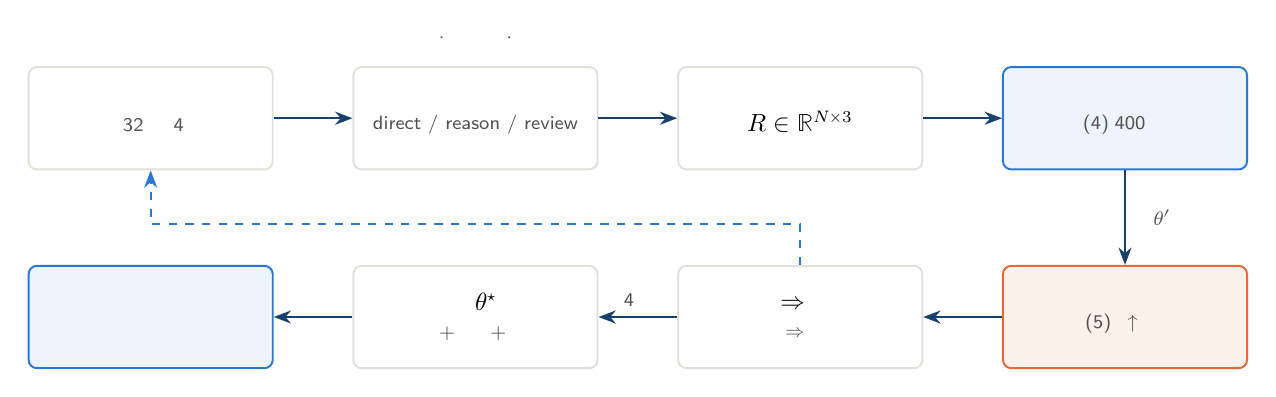
\begin{tikzpicture}[
  font=\sffamily\small, node distance=7mm and 10mm,
  box/.style={draw=hair, fill=white, rounded corners=3pt, align=center, inner sep=4pt,
              minimum height=13mm, minimum width=31mm, line width=0.7pt},
  hl/.style={box, fill=accentwash, draw=accent},
  gate/.style={box, fill=warmwash, draw=warm},
  arr/.style={-{Stealth[length=2.2mm]}, line width=0.8pt, color=accentdark},
  lbl/.style={font=\sffamily\scriptsize, text=ink2}]
  \node[box] (batch) {新一批训练题\\[-1pt]{\scriptsize\color{ink2}每轮 32 题，共 4 轮}};
  \node[box, right=of batch] (collect) {全动作采集\\[-1pt]{\scriptsize\color{ink2}direct / reason / review}};
  \node[box, right=of collect] (matrix) {累计奖励矩阵\\[-1pt]$R\in\mathbb{R}^{N\times 3}$};
  \node[hl, right=of matrix] (grad) {精确梯度上升\\[-1pt]{\scriptsize\color{ink2}式 (4)，400 步，暖启动}};
  \node[gate, below=12mm of grad] (gatebox) {验证门控\\[-1pt]{\scriptsize\color{ink2}式 (5)：效用↑ 且准确率守卫}};
  \node[box, left=of gatebox] (accept) {接纳 $\Rightarrow$ 更新现任\\[-1pt]{\scriptsize\color{ink2}拒绝 $\Rightarrow$ 保留现任}};
  \node[box, left=of accept] (freeze) {冻结 $\theta^\star$\\[-1pt]{\scriptsize\color{ink2}参数 + 配置哈希 + 时间戳}};
  \node[hl, left=of freeze] (test) {独立测试集\\[-1pt]{\scriptsize\color{ink2}冻结后一次性评测}};
  \node[lbl, above=1.5mm of collect] {预算账本 · 防重复计费缓存 · 共享初稿};
  \draw[arr] (batch) -- (collect);
  \draw[arr] (collect) -- (matrix);
  \draw[arr] (matrix) -- (grad);
  \draw[arr] (grad) -- node[lbl, right] {候选 $\theta'$} (gatebox);
  \draw[arr] (gatebox) -- (accept);
  \draw[arr] (accept) -- node[lbl, above] {4 轮后} (freeze);
  \draw[arr] (freeze) -- (test);
  \draw[arr, color=accent, dashed] (accept.north) -- ++(0,5.2mm) -| node[lbl, pos=0.25, above] {下一轮} (batch.south);
\end{tikzpicture}
\caption{GFPG 的增量自我改进流程。只有通过门控的候选才会成为现任；四轮结束后先写入冻结文件，之后才首次请求测试集。}
\label{fig:pipeline}
\end{figure}

\begin{algorithm}[t]
\caption{GFPG：门控全信息策略梯度的增量自我改进}\label{alg:gfpg}
\KwIn{按批到达的训练题（$K=\numRounds$ 批），验证集 $\mathcal{D}_{\mathrm{val}}$，步长 $\eta$，每轮步数 $S$，正则系数 $\tau,\lambda$，容差 $\epsilon=\numGateTol$}
\KwOut{冻结的路由器 $\theta^\star$，验证集选出的最佳固定动作 $a^\dagger$}
采集验证集每题三条动作的结果，得到 $R^{\mathrm{val}}$\;
$\theta_0\leftarrow(W=0,\ b=(0,0.5,0))$；$\theta_{\mathrm{inc}}\leftarrow\theta_0$；$\mathcal{H}\leftarrow\varnothing$ \tcp*{初始：总是 reason}
\For{$k\leftarrow1$ \KwTo $K$}{
  对第 $k$ 批每题执行 direct、reason、review（复用 reason 初稿），记录正确性与 token\;
  $\mathcal{H}\leftarrow\mathcal{H}\cup\{\text{第 }k\text{ 批}\}$，按式 \eqref{eq:reward} 构造累计奖励矩阵 $R$\;
  $\theta'\leftarrow\theta_{\mathrm{inc}}$ \tcp*{暖启动}
  \For{$s\leftarrow1$ \KwTo $S$}{
    $\theta'\leftarrow\theta'+\eta\,\nabla_\theta J(\theta';R)$ \tcp*{式 \eqref{eq:grad}，精确梯度}
  }
  \eIf{$\theta'$ 满足门控条件 \eqref{eq:gate}}{
    $\theta_{\mathrm{inc}}\leftarrow\theta'$ \tcp*{接纳}
  }{
    保留 $\theta_{\mathrm{inc}}$，存档 $\theta'$ \tcp*{拒绝并回退}
  }
}
$a^\dagger\leftarrow\arg\max_a U_{\mathrm{val}}(\text{固定 }a)$\;
写入冻结文件（参数、版本号、$a^\dagger$、配置哈希、时间戳），\textbf{之后}才请求测试集\;
\Return{$\theta^\star=\theta_{\mathrm{inc}}$，$a^\dagger$}
\end{algorithm}

\subsection{工程实现要点}\label{sec:engineering}
\begin{itemize}
  \item \textbf{预算账本}：每次 HTTP 调用\emph{之前}先写入并 \code{fsync} 一条 attempt 记录；失败重试同样计入上限；进程重启从账本恢复计数，不会重置预算。
  \item \textbf{防重复计费缓存}：缓存键为“接口地址 + 模型 + 消息 + 参数”的 SHA-256；同一请求并发时只发一次；缓存文件损坏时拒绝自动付费重请求。
  \item \textbf{共享初稿}：\act{review} 复用同题 \act{reason} 的输出作为第一步，采集成本为每题 3 次；但部署成本始终按两次调用累计，不因缓存而少算。
  \item \textbf{冻结与一致性}：配置记录超参数、数据 SHA-256 与实现文件哈希；冻结文件先于任何测试请求写入；配置或实现变化时拒绝复用旧结果。
  \item \textbf{离线复核}：\code{scripts/replay_report.py} 不读密钥、不调用模型，重算评分、token 账、门控决策、测试指标与 bootstrap，并逐项比对。
  \item \textbf{密钥安全}：API 密钥只写入权限为 0600 的临时 header 文件，不出现在命令行参数、缓存或账本中。
\end{itemize}

% =============================================================================
\section{AI 辅助设计过程}\label{sec:ai}
% =============================================================================

本项目在 AI 编程助手（大语言模型代理）辅助下完成。我们把 AI 的作用限定为“提出、推导、实现、检查”，把目标设定、约束与最终判断留给人，
并要求 AI 的每一类产出都有可执行的核查手段。

\subsection{人机分工}
\begin{table}[H]
\centering\small
\caption{各环节的人机分工与留存证据}\label{tab:ai}
\begin{tabularx}{\linewidth}{@{}>{\raggedright\arraybackslash\sffamily\bfseries}p{1.7cm}LL>{\raggedright\arraybackslash}p{3.3cm}@{}}
\toprule
环节 & AI 助手的工作 & 人的职责 & 仓库中的证据 \\
\midrule
问题筛选 & 归纳候选问题（过度推理、盲目复核、静态路由）并评估可测性与成本 & 确定研究问题与约 1000 次的总请求预算、指定模型接口 & \code{research_plan.md} \S1 \\
方法推导 & 推导含熵正则的 softmax 策略梯度；提出以全信息反馈替代动作采样 & 审核推导，要求逐分量数值验证 & \code{policy.py}、\code{test_policy.py} \\
实验设计 & 设计划分、门控规则、最佳固定基线、oracle 诊断与配对 bootstrap & 确认“测试前冻结、不按测试结果调参”等规则 & \code{research_plan.md} \S4–\S8 \\
工程实现 & 编写 harness、预算账本、缓存、冻结、离线复核与单元测试 & 运行测试；在本地提供 API 凭据（不入库） & \code{harness_rsi/}、\code{tests/} \\
执行排障 & 遇到 HTTP 429 后加入全局节流与冷却；截断的空回答按答错计分并保留成本 & 确认修复发生在任何训练采集与测试之前 & \code{config_history/} \\
结果解释 & 生成报告并强制与最佳固定策略比较；补充检查严格标注为探索性 & 接受负面结论，不挑选有利基线 & \code{findings.md}、本报告 \\
\bottomrule
\end{tabularx}
\end{table}

\subsection{关键设计迭代}
\begin{enumerate}[label=(\arabic*)]
  \item \textbf{从“文本梯度”到数值梯度}：TextGrad 式反馈无法做有限差分验证，也难以用课程中的收敛工具分析；因此改为对路由参数求解析梯度。
  \item \textbf{从采样梯度到全信息精确梯度}：动作只有 3 条，且 \act{review} 可复用 \act{reason} 初稿，测全部动作每题只需 3 次请求；
        换来的是零采样方差的梯度（图~\ref{fig:method}b 量化了这一点）。
  \item \textbf{门控从“相对现任”扩展为“相对初始与现任的较高者”}：防止多轮小幅下降累积成大幅退化。
  \item \textbf{传输层修复}：服务端限流后加入全局节流与冷却；修复发生在训练采集与最终测试之前，旧配置哈希保留在 \code{config_history/}，题目与提示词未变。
  \item \textbf{结果审计}：发现学习路由器未超过最佳固定策略后，没有替换主结论或更换基线；额外的 \numConvSteps{} 步收敛检查被严格标注为探索性分析。
\end{enumerate}

\subsection{如何核查 AI 的产出}
\begin{keybox}{核查原则：AI 的每一类产出都对应一种可执行的检验}
\begin{itemize}[leftmargin=1.3em]
  \item \textbf{数学推导} $\to$ 中心差分逐分量比对解析梯度：\numGradParams{} 个参数的最大绝对误差为 $\numGradMaxErr$（图~\ref{fig:method}a）。
  \item \textbf{代码行为} $\to$ \numUnitTests{} 项单元测试：预算并发下不可超支、缓存命中不计费、仅对 429/5xx 重试且每次计数、答案严格解析、报告生成格式等。
  \item \textbf{实验数值} $\to$ 离线复核脚本重算全部 \numTotalTasks{} 题、\numSuccesses{} 次成功请求的 token 账与所有指标，并逐项比对。
  \item \textbf{结论表述} $\to$ 预先写定的解释规则（\code{research_plan.md} \S8）：配对区间跨 0 时只能写“证据不足”。
\end{itemize}
\end{keybox}

% =============================================================================
\section{实验设置}\label{sec:setup}
% =============================================================================

\paragraph{数据。}使用 GSM8K\cite{gsm8k} 官方完整数据（train 7{,}473 行、test 1{,}319 行，逐行校验并记录 SHA-256）。
训练与验证题只从官方 train 抽取，测试题只从官方 test 抽取；按规范化题面哈希去重，并剔除 train/test 间重复题。
固定种子 \numSeed{} 抽样，不按难度或模型表现筛题：训练 \numTrainN{}、验证 \numValN{}、测试 \numTestN{}，共 \numTotalTasks{} 题。

\paragraph{模型与调用。}通过 OpenAI 兼容的 \code{/v1/chat/completions} 接口调用 \code{deepseek-v4.1-flash}，温度 0，单次最大输出 \numMaxTokens{} token。
无失败时需要 $3\times\numTotalTasks=912$ 次请求；本次运行的请求尝试上限为 \numMaxRequests{}。

\begin{table}[H]
\centering\small
\caption{超参数（全部在实验前固定）}\label{tab:hparams}
\begin{tabularx}{\linewidth}{@{}lLlL@{}}
\toprule
参数 & 取值 & 参数 & 取值 \\
\midrule
特征维数 / 参数量 & \numFeatures{} / \numParams{} & 成本权重 $\kappa$ & \numCostWeight{}（每 1000 token） \\
熵系数 $\tau$ & \numEntropy{} & $L_2$ 系数 $\lambda$ & \numLtwo{}（偏置不正则） \\
学习率 $\eta$ & \numLR{}（全批量） & 每轮步数 $S$ & \numSteps{} \\
轮数 × 每批题数 & \numRounds{} × 32 & 初始策略 & $W=0,\ b=(0,0.5,0)$，即总是 \act{reason} \\
门控效用裕量 & $10^{-6}$ & 门控准确率容差 & \numGateTol{}（相对初始与现任的较高者） \\
请求尝试上限 & \numMaxRequests{}（含失败重试） & 部署规则 & $\arg\max$，温度 0 \\
\bottomrule
\end{tabularx}
\end{table}

\paragraph{基线与指标。}主要比较为“学习路由器 $-$ 验证集选出的最佳固定路线”；辅助比较包括初始 \act{reason}、三条固定路线、
均匀随机路由的期望指标，以及使用测试标签逐题选最优动作的 oracle（不可部署，仅作上界）。指标为准确率、平均 token、平均调用数、平均延迟与效用。

\paragraph{统计方法。}在同一批 \numTestN{} 道测试题上逐题计算差值，用 5000 次按题配对的 bootstrap 求 95\% 百分位区间\cite{efron1993}；
每次重采样对两种策略使用同一组题目索引，保留同题相关性。解释规则在实验前写定：效用差区间下界大于 0 才称“取得正向证据”，跨 0 则称“证据不足”。

% =============================================================================
\section{实验结果}\label{sec:results}
% =============================================================================

\subsection{方法正确性验证}\label{sec:verify}
图~\ref{fig:method}(a) 在真实训练特征与奖励上随机取参数点，对 \numGradParams{} 个参数逐一做中心差分（$\varepsilon=10^{-6}$）：
解析梯度与数值梯度几乎完全重合，最大绝对误差 $\numGradMaxErr$。

图~\ref{fig:method}(b) 量化了“全信息”带来的好处：在 v1 初始策略处，用已记录的奖励矩阵离线模拟 REINFORCE，并按真实 API 调用计费
（温度 0 下重复采样同一动作命中缓存、不再计费；\act{review} 复用已采样的 \act{reason} 初稿）。每题 1 个采样时约需 \numReinforceCalls{} 次调用，
梯度方向与精确梯度的平均余弦仅约 \numReinforceCos{}；即使每题采样 16 次、调用数（约 383 次）已接近全信息采集的 \numExactCalls{} 次，平均余弦也只有约 0.76，且波动很大。
GFPG 以 \numExactCalls{} 次调用得到方向完全准确（余弦为 1）、无方差的梯度。

\begin{figure}[t]
\centering
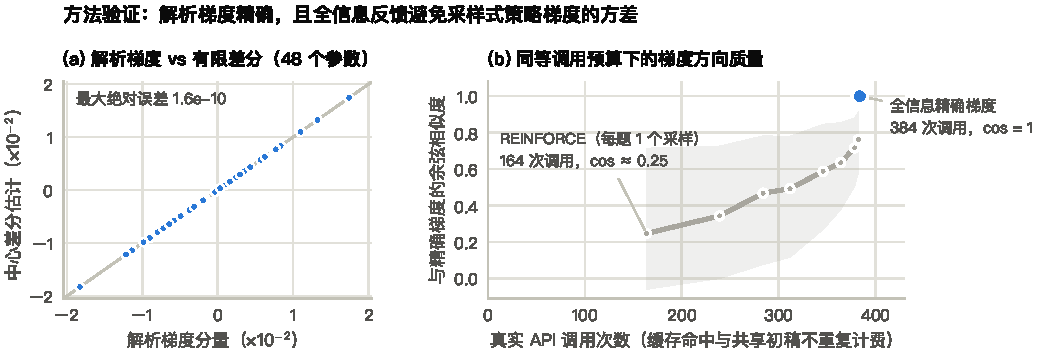
\includegraphics[width=\linewidth]{fig_gradient_method.pdf}
\caption{方法验证（离线，未新增 API 调用）。(a) 解析梯度与中心差分逐分量比较；(b) 同等真实调用预算下，REINFORCE 估计与精确梯度的余弦相似度
（灰线为 400 次重复的均值，灰带为 10\%–90\% 分位）。}
\label{fig:method}
\end{figure}

为检验方法在“确有路由空间”时能否学到依赖上下文的决策，图~\ref{fig:synthetic} 复现了单元测试中的合成任务：二维特征，左半平面动作 A 最优、右半平面动作 B 最优。
精确梯度上升 350 步后，目标 $J$ 单调上升，最优动作的平均概率升至 0.91，未见输入上的正确路由率为 \numSyntheticAcc\%。该实验只说明方法机制可行，不代表真实基准上的收益。

\begin{figure}[t]
\centering
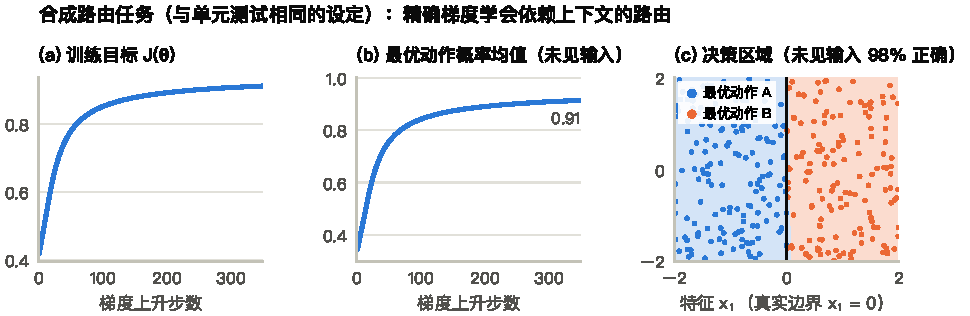
\includegraphics[width=\linewidth]{fig_synthetic.pdf}
\caption{合成路由任务（与 \code{tests/test_policy.py} 相同的设定）。(c) 背景色为学到的决策区域，散点为未见输入按真实最优动作着色，黑线为真实边界。}
\label{fig:synthetic}
\end{figure}

\subsection{独立测试集主结果}
表~\ref{tab:main} 与图~\ref{fig:main} 给出冻结策略在 \numTestN{} 道独立测试题上的表现。

\begin{table}[H]
\centering\small
\caption{独立测试集结果（\numTestN{} 题；token 变化相对初始 \act{reason}；$^\dagger$ oracle 使用测试标签，不可部署）}\label{tab:main}
\setlength{\tabcolsep}{4.2pt}
\begin{tabularx}{\linewidth}{@{}Lccccccc@{}}
\toprule
策略 & 答对 & 正确率 & 平均 token & token 变化 (\%) & 调用数 & 延迟 (s) & 效用 \\
\midrule
\inputrows{generated/table_main.tex}
\bottomrule
\end{tabularx}
\end{table}

\begin{figure}[t]
\centering
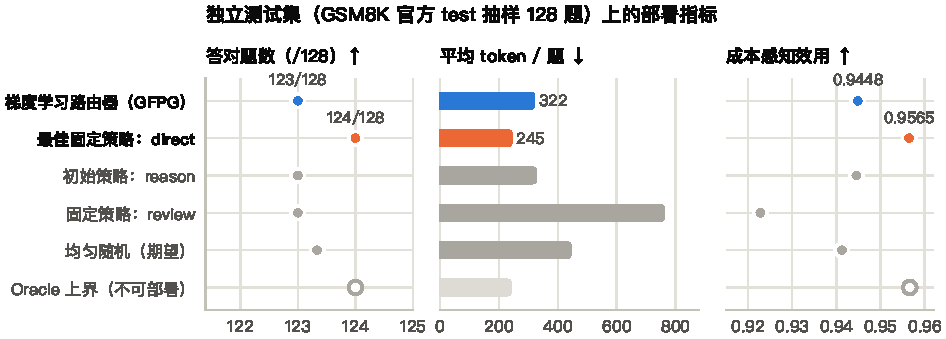
\includegraphics[width=\linewidth]{fig_main_results.pdf}
\caption{测试集部署指标。蓝色为 GFPG 冻结路由器，橙色为验证集选出的最佳固定策略，灰色为其他基线；空心点为不可部署的 oracle。
效用 $=$ 正确率 $-\,\numCostWeight\times$token$/1000$。答对题数轴未从 0 开始，以便看清一题之差。}
\label{fig:main}
\end{figure}

\begin{itemize}
  \item \textbf{GFPG 路由器}：答对 \numLearnedCorrect{}/\numTestN{}，与初始流程相同；平均 token 从 \numInitTokens{} 降至 \numLearnedTokens{}（\numLearnedTokenChange\%）。
        它对 \numPickDirect{} 题选择 \act{direct}、\numPickReason{} 题选择 \act{reason}，从不选择 \act{review}。
  \item \textbf{最佳固定策略 \act{direct}}（由验证集选出）：答对 \numBestCorrect{}/\numTestN{}，平均 token 仅 \numBestTokens{}（\numBestTokenChange\%），效用最高的可部署方案。
  \item \textbf{固定 \act{review}}：准确率与 \act{reason} 相同，但 token 增加 \numReviewTokenChange\%；复核纠正错误 \numReviewFixes{} 次、改错正确答案 \numReviewBreaks{} 次。
  \item \textbf{Oracle}：答对 \numOracleCorrect{}/\numTestN{}，与固定 \act{direct} 相同，只比它再省 \numOracleExtraTokens{} token/题（\numOracleExtraPct\%）。
\end{itemize}

\subsection{配对统计检验}
\begin{table}[H]
\centering\small
\caption{学习路由器 $-$ 对照的逐题配对差值（点估计与 95\% bootstrap 区间；准确率以百分点计）}\label{tab:paired}
\setlength{\tabcolsep}{3.6pt}
\begin{tabularx}{\linewidth}{@{}Lccccccc@{}}
\toprule
\multirow{2}{*}{对照} & \multicolumn{2}{c}{$\Delta$ 正确率（pp）} & \multicolumn{2}{c}{$\Delta$ token / 题} & \multicolumn{2}{c}{$\Delta$ 效用} & \multirow{2}{*}{效用结论} \\
\cmidrule(lr){2-3}\cmidrule(lr){4-5}\cmidrule(lr){6-7}
 & 点估计 & 95\% 区间 & 点估计 & 95\% 区间 & 点估计 & 95\% 区间 & \\
\midrule
\inputrows{generated/table_paired.tex}
\bottomrule
\end{tabularx}
\end{table}

\begin{figure}[t]
\centering
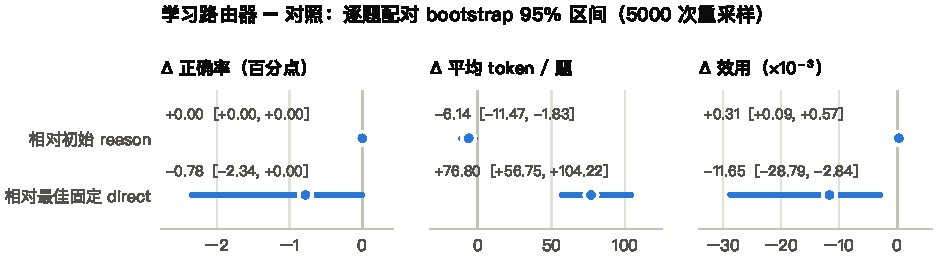
\includegraphics[width=\linewidth]{fig_paired_ci.pdf}
\caption{逐题配对 bootstrap 95\% 区间。竖线为 0；区间不跨 0 表示差异在本测试分布与成本权重下可分辨。}
\label{fig:paired}
\end{figure}

\begin{keybox}{结论一：相对初始 harness，GFPG 带来统计上可分辨的小幅改进}
两者在 \numTestN{} 道题上的逐题正确性完全相同（准确率差恒为 0），而 token 差为 \numVsInitTok{}，95\% 区间 \numVsInitTokCI{}；
效用差 \numVsInitUtil{}，区间 \numVsInitUtilCI{}，均不含 0。即：自我改进循环在不损失任何一道题的前提下，稳定地节省了少量 token。
\end{keybox}

\begin{warnbox}{结论二：GFPG 显著劣于验证集选出的最佳固定策略}
相对固定 \act{direct}，效用差为 \numVsBestUtil{}，95\% 区间 \numVsBestUtilCI{} 完全位于 0 以下；每题多用 \numVsBestTok{} token。
准确率差 \numVsBestAcc{} 个百分点的区间 \numVsBestAccCI{} 含 0，因此不把 \act{direct} 多答对的 1 题宣称为显著的准确率优势。
\textbf{在当前模型与基准下，实际部署更推荐固定 \act{direct}}；冻结的梯度路由器作为完整、可复现的方法实验保留。
\end{warnbox}

\subsection{自我改进过程}
\begin{table}[H]
\centering\small
\caption{四轮自我改进记录（$J$ 为训练代理目标；“决策变化”为候选与现任在验证集上 $\arg\max$ 不同的题数）}\label{tab:rounds}
\begin{tabularx}{\linewidth}{@{}cc>{\centering\arraybackslash}X>{\centering\arraybackslash}Xcccc@{}}
\toprule
轮次 & 累计训练题 & $J$ 起点 & $J$ 终点 & 现任验证效用 & 候选验证效用 & 决策变化 & 门控 \\
\midrule
\inputrows{generated/table_rounds.tex}
\bottomrule
\end{tabularx}
\end{table}

\begin{figure}[t]
\centering
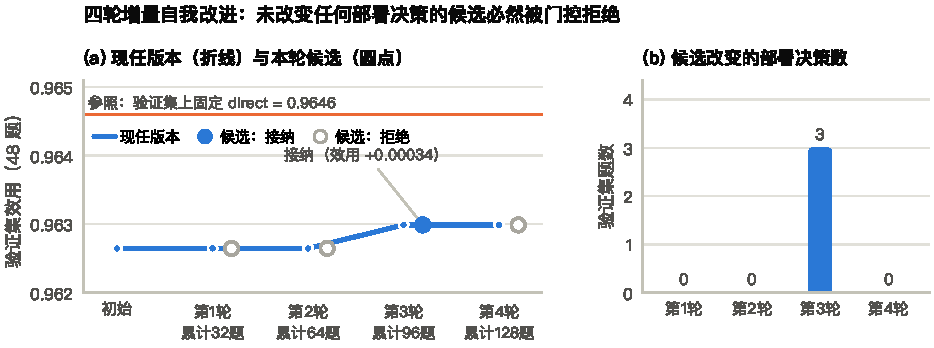
\includegraphics[width=\linewidth]{fig_rounds.pdf}
\caption{自我改进过程。(a) 验证集效用：折线为每轮结束后的现任版本，圆点为本轮候选；(b) 候选相对现任改变的验证集部署决策数（由已存档的候选参数重算）。}
\label{fig:rounds}
\end{figure}

每轮梯度上升都提升了训练目标 $J$，但幅度很小。更关键的是图~\ref{fig:rounds}(b)：第 1、2、4 轮的候选在验证集上与现任\emph{做出完全相同的部署决策}，
验证效用因此毫无变化，只能被门控拒绝；只有第 3 轮候选把 \numAcceptedValChanged{} 道验证题从 \act{reason} 改为 \act{direct}，效用提升 0.00034 而被接纳，成为最终冻结的版本 \numSelectedVersion{}。
我们把这种“改变了概率、却没有改变任何 $\arg\max$ 决策”的更新称为\textbf{决策不可见的更新}，它是本实验中自我改进幅度受限的直接原因之一（\S\ref{sec:why}）。

\subsection{成本与预算}
\begin{figure}[t]
\centering
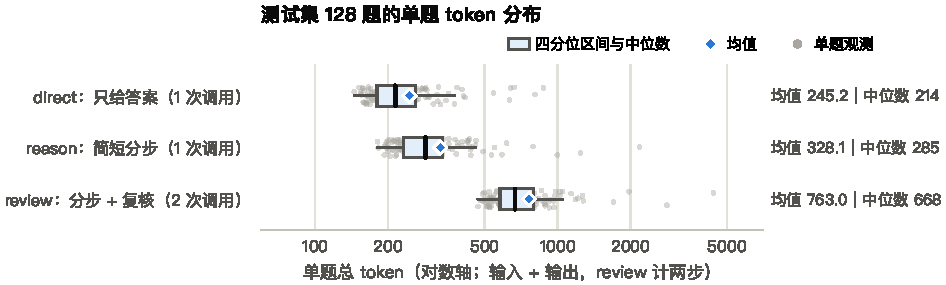
\includegraphics[width=\linewidth]{fig_tokens.pdf}
\caption{测试集单题 token 分布（对数轴）。\act{review} 的成本约为 \act{reason} 的 2.3 倍，却没有纠正任何错误。}
\label{fig:tokens}
\end{figure}

\begin{figure}[t]
\centering
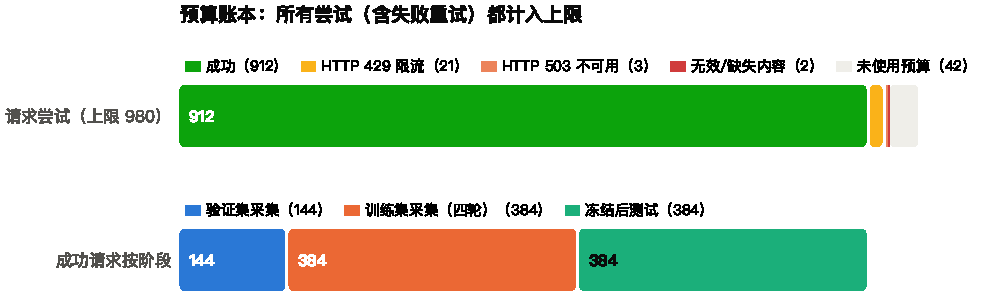
\includegraphics[width=\linewidth]{fig_budget.pdf}
\caption{请求账本。上：全部尝试（含失败重试）相对上限 \numMaxRequests{}；下：成功请求按阶段分解（与上方“成功”段同一比例尺）。}
\label{fig:budget}
\end{figure}

\begin{table}[H]
\centering\small
\caption{请求与 token 账本}\label{tab:requests}
\begin{tabularx}{0.78\linewidth}{@{}Xr@{}}
\toprule
项目 & 次数 \\
\midrule
\inputrows{generated/table_requests.tex}
\bottomrule
\end{tabularx}
\end{table}

主实验共尝试 \numAttempts{} 次请求：成功 \numSuccesses{} 次、失败 \numFailures{} 次（以 HTTP 429 限流为主）；加上 1 次早期连通性探测，共 \numCombinedAttempts{} 次，
低于约 1000 次的授权上限。成功响应共记录 \numTotalTokens{} token（输入 \numInputTokens{}，输出 \numOutputTokens{}）；失败请求若被供应商计费，其费用无法从日志还原。
若未来题目分布与质量保持不变，按每题节省 \numSavedPerTask{} token 计算，需要约 \numAmortize{} 道后续题目才能摊销全部采集 token——这是有条件的估算，而非已获得的净收益。

% =============================================================================
\section{分析与讨论}\label{sec:discussion}
% =============================================================================

\subsection{GFPG 在哪些方面是有效的}
\begin{enumerate}[label=(\arabic*)]
  \item \textbf{梯度精确、计算廉价}：解析梯度经逐分量有限差分验证；\numParams{} 个参数的全批量更新在 CPU 上为毫秒级，无需 GPU。
  \item \textbf{全信息优于采样}：在相同调用预算下，采样式策略梯度的方向噪声很大（余弦约 \numReinforceCos{}–0.76），而全信息梯度没有采样方差。
  \item \textbf{自我改进循环按设计工作}：只有改变了部署决策且通过门控的候选被接纳；冻结版本相对初始 harness 取得 CI 不含 0 的 token 节省，且逐题零准确率损失。
  \item \textbf{工程可信}：\numAttempts{} 次请求未超预算；测试请求全部发生在冻结之后；全部指标可离线复核。
\end{enumerate}

\subsection{为什么没有超过最佳固定策略}\label{sec:why}
\paragraph{(1) 路由空间几乎不存在。}oracle 与固定 \act{direct} 答对题数相同，只多省 \numOracleExtraPct\% 的 token。
这意味着测试集上 \act{direct} 答错的 \numTestAllWrong{} 题，\act{reason} 与 \act{review} 也全部答错——三条路线在正确性上没有互补，
而 \act{direct} 在 \numTestDirectCheaperPct\% 的题上比 \act{reason} 更省 token。任何路由器的上限都只比“总是 \act{direct}”高出约 0.0002 的效用。

\paragraph{(2) 训练数据把学习引向 \act{reason}。}在 \numTrainN{} 道训练题中，只有 \numTrainFlipToReason{} 题出现“\act{direct} 错而 \act{reason} 对”，
反向情形为 \numTrainFlipToDirect{} 题；但一题正确性的差别（$1/128\approx0.0078$）超过了 \act{direct} 平均节省 token 带来的效用（约 0.004）。
于是在训练集上固定 \act{reason} 的效用（\numTrainReasonUtil{}）反而高于固定 \act{direct}（\numTrainDirectUtil{}），梯度自然把路由器推向 \act{reason}。
在验证集上两者没有正确性差异（固定 \act{direct} 效用 \numValDirectUtil{}，\act{reason} \numValReasonUtil{}），测试集上则是反向的 \numTestFlipToDirect{} 题。
单题翻转这种稀有、大幅度的奖励差异，是小样本 harness 优化中最需要警惕的噪声来源。

\paragraph{(3) 步长预算不足导致“决策不可见的更新”。}每轮 \numSteps{} 步、学习率 \numLR{} 的全批量梯度上升只让 logit 产生很小的变化，
4 轮中有 \numRejectedNoChange{} 轮候选没有改变任何验证集决策。仓库中另存的一次 \numConvSteps{} 步收敛检查（只用前 64 道训练题与验证集）
得到的路由在 \numValN{} 道验证题上全部选择 \act{direct}，验证效用 \numConvUtil{}，与固定 \act{direct} 相同。
该检查是在看到早期验证结果后追加的，且冻结时间晚于第一次测试请求，因此只作为探索性证据，不替换原方案的结论（见 \code{artifacts/convergence_check/NOTE.md}）。

\subsection{复核为何无效}
固定 \act{review} 在测试集上纠正 \numReviewFixes{} 题、改错 \numReviewBreaks{} 题，却让 token 增加 \numReviewTokenChange\%。
基础模型在 GSM8K 上的准确率已超过 96\%，剩余错误多为三条路线同时答错的题，复核难以改变答案。
此外 \act{reason} 与 \act{review} 各有 \numFormatFailReason{} 题因输出截断而未给出有效答案（\act{direct} 为 \numFormatFailDirect{} 题），均按答错计分并保留其 token 成本。

\subsection{对 RSI Harness 工程的启示}
\begin{keybox}{四条可迁移的经验}
\begin{enumerate}[label=\arabic*.,leftmargin=1.4em]
  \item \textbf{永远与“验证集选出的最佳固定配置”比较}：只和初始配置比，会把“选对一个固定流程”的收益误认为自适应的功劳。
  \item \textbf{先测路由空间，再加控制复杂度}：oracle 与最佳固定策略差距很小时，复杂路由器只会增加估计误差。
  \item \textbf{让自我修改“决策可见”}：步长与停止准则应以部署决策是否改变为参照，而不仅是代理目标是否上升。
  \item \textbf{预算账本与冻结协议是诚实评估的前提}：失败重试计费、测试前冻结、离线复核，使正负结果都可被他人核验。
\end{enumerate}
\end{keybox}

% =============================================================================
\section{局限性与后续工作}\label{sec:limits}
% =============================================================================

\paragraph{局限性。}仅一个模型、一个公开基准子集与一个训练种子；测试集 \numTestN{} 题，一题即 0.78 个百分点；每个（题目，动作）只有一次观测，温度 0 也不保证服务端完全确定；
GSM8K 是公开数据，无法排除预训练污染；同一验证集被用于 4 次门控，存在自适应选择；bootstrap 区间只反映题目抽样的不确定性，不覆盖模型版本或服务端随机性；token 不等于货币成本。

\paragraph{后续工作。}
\begin{enumerate}[label=(\arabic*)]
  \item \textbf{自适应步长}：引入 Armijo 回溯线搜索、自然梯度（Fisher 预条件）或 Adam，并以“部署决策是否改变”作为每轮更新的检查点，避免决策不可见的更新。
  \item \textbf{稳健的奖励估计}：对稀有的正确性翻转做收缩或影响力限制，降低单题噪声对梯度方向的支配。
  \item \textbf{引入真正互补的动作}：例如调用计算器 / 代码执行、检索等；先在新的开发集上测量 oracle 空间，确有互补性再训练路由器。
  \item \textbf{确认性评估}：在从未用于探索的新测试集上，与验证集最佳固定策略和成本感知启发式做一次性比较；扩展到多模型、多种子与成本权重敏感性分析。
\end{enumerate}

% =============================================================================
\section{结论}\label{sec:conclusion}
% =============================================================================
本文在 AI 辅助下设计并实现了面向 LLM Harness 受限自我改进的梯度类方法 GFPG。它利用全信息反馈把策略梯度变为可解析、可验证、零采样方差的精确梯度，
并通过带累计准确率守卫的验证门控与测试前冻结，构成一个预算受控、可审计的自我改进循环。在 \numAttempts{} 次真实 API 请求的实验中，
GFPG 相对初始 harness 取得了统计上可分辨、零准确率损失的小幅 token 节省；但它没有超过验证集选出的固定 \act{direct} 策略，
oracle 诊断表明该基准上几乎不存在可供路由利用的空间。我们认为，这一“方法正确、收益有限、原因清楚”的完整结果，
比只展示训练目标上升更能说明梯度类方法在真实 harness 自我改进中的价值与边界。

% =============================================================================
\begin{thebibliography}{99}
\small
\setlength{\itemsep}{2pt}
\bibitem{williams1992} R.~J. Williams. Simple statistical gradient-following algorithms for connectionist reinforcement learning. \emph{Machine Learning}, 8(3–4):229–256, 1992.
\bibitem{sutton2000} R.~S. Sutton, D.~McAllester, S.~Singh, Y.~Mansour. Policy gradient methods for reinforcement learning with function approximation. In \emph{Advances in Neural Information Processing Systems 12}, 2000.
\bibitem{mei2020} J.~Mei, C.~Xiao, C.~Szepesvári, D.~Schuurmans. On the global convergence rates of softmax policy gradient methods. In \emph{ICML}, 2020.
\bibitem{nocedal2006} J.~Nocedal, S.~J. Wright. \emph{Numerical Optimization}, 2nd ed. Springer, 2006.
\bibitem{gsm8k} K.~Cobbe, V.~Kosaraju, M.~Bavarian, et~al. Training verifiers to solve math word problems. arXiv:2110.14168, 2021.
\bibitem{textgrad} M.~Yuksekgonul, F.~Bianchi, J.~Boen, S.~Liu, Z.~Huang, C.~Guestrin, J.~Zou. TextGrad: Automatic “differentiation” via text. arXiv:2406.07496, 2024.
\bibitem{adas} S.~Hu, C.~Lu, J.~Clune. Automated design of agentic systems. arXiv:2408.08435, 2024.
\bibitem{gepa} L.~A. Agrawal, et~al. GEPA: Reflective prompt evolution can outperform reinforcement learning. arXiv:2507.19457, 2025.
\bibitem{dgm} J.~Zhang, S.~Hu, C.~Lu, R.~Lange, J.~Clune. Darwin Gödel Machine: Open-ended evolution of self-improving agents. arXiv:2505.22954, 2025.
\bibitem{grpo} Z.~Shao, P.~Wang, Q.~Zhu, et~al. DeepSeekMath: Pushing the limits of mathematical reasoning in open language models. arXiv:2402.03300, 2024.
\bibitem{efron1993} B.~Efron, R.~J. Tibshirani. \emph{An Introduction to the Bootstrap}. Chapman \& Hall/CRC, 1993.
\end{thebibliography}

% =============================================================================
\appendix
\ctexset{section/name={附录\,,}, section/number=\Alph{section}}
% =============================================================================
\section{复现指南}\label{app:repro}
需要 Python 3.10+、NumPy 与系统 \code{curl}。以下命令在仓库根目录执行（Windows PowerShell 同样适用，环境变量写法见 README）。

\begin{tcolorbox}[enhanced, colback=accentwash!60!white, colframe=hair, boxrule=0.6pt, arc=2pt, left=8pt, right=8pt, top=4pt, bottom=4pt,
                  fontupper=\ttfamily\small]
\# 1. Install the only runtime dependency and run the unit tests\\
python -m pip install -r requirements.txt\\
python -m unittest discover -s tests -v\\[4pt]
\# 2. Re-verify every recorded number offline (no API key, no model call)\\
python scripts/replay\_report.py --run artifacts/gsm8k\_flash\_v1\\[4pt]
\# 3. Re-draw the report figures and tables (needs matplotlib)\\
python -m pip install -r requirements-report.txt\\
python scripts/make\_figures.py\\[4pt]
\# 4. Re-build this PDF (XeLaTeX + ctex), then copy it to the repository root\\
cd report \&\& latexmk -xelatex main.tex \&\& cp main.pdf ../REPORT.pdf\\[4pt]
\# 5. Optional: rerun the real-API experiment (needs your own key; costs requests)\\
export HARNESS\_BASE\_URL=https://your-provider.example/v1\\
export HARNESS\_MODEL=your-model HARNESS\_API\_KEY=...\\
python scripts/download\_data.py\\
python -m harness\_rsi.experiment --output artifacts/my\_run --max-requests 980 --workers 4
\end{tcolorbox}

离线复核会校验实现文件哈希、数据划分、逐题评分、逐请求 token 账、冻结策略、每轮门控、测试指标、配对 bootstrap 与预测导出，全部通过时输出 \code{verified_offline}。

\section{仓库结构}\label{app:tree}
\begin{table}[H]
\centering\small
\begin{tabularx}{\linewidth}{@{}>{\ttfamily}p{5.0cm}L@{}}
\toprule
路径 & 内容 \\
\midrule
REPORT.pdf & 本报告（课程提交用 PDF） \\
README.md & 项目说明、关键结果与快速开始 \\
harness\_rsi/ & 核心实现：client（预算与缓存）、tasks、strategies、policy（梯度）、experiment、evaluation、report \\
scripts/ & 数据下载、离线复核、作图、冻结策略推理、探索性收敛检查 \\
tests/ & 单元测试（梯度、预算、缓存、评分、门控、报告生成） \\
artifacts/gsm8k\_flash\_v1/ & 真实实验：配置、逐题观测、请求账本、各轮候选、冻结策略、测评报告 \\
artifacts/convergence\_check/ & 探索性 \numConvSteps{} 步收敛检查（如实标注，不替换主结论） \\
docs/ & 研究计划、结果讨论、来源核验记录 \\
report/ & 本报告的 LaTeX 源码、图表与自动生成的数值表 \\
\bottomrule
\end{tabularx}
\end{table}

\section{自动化测试清单}\label{app:tests}
\begin{table}[H]
\centering\small
\caption{单元测试覆盖（\code{python -m unittest discover -s tests}）}\label{tab:tests}
\begin{tabularx}{\linewidth}{@{}>{\ttfamily}p{3.6cm}cL@{}}
\toprule
文件 & 数量 & 覆盖内容 \\
\midrule
test\_policy.py & \numTestsPolicy{} & 解析梯度 vs 有限差分；合成任务上学会上下文路由；标准化冻结与序列化；数值稳定的 softmax；特征不依赖答案；拒绝不完整奖励矩阵 \\
test\_client.py & \numTestsClient{} & 缓存命中不计费且预算跨重启保留；并发下预算不超支；相同请求只发一次；缺失 / 零 usage 视为失败；仅对 429/5xx 重试且计数；截断空回答保留成本；全局节流与 429 冷却；密钥不进命令行 \\
test\_evaluation.py & \numTestsEvaluation{} & 指标与效用公式；随机策略的期望指标；相同策略的配对区间恰为 0；差值符号与种子可复现；非法输入拒绝 \\
test\_tasks.py & \numTestsTasks{} & 数值解析与精确比较；不从推理过程猜答案；最后一个显式答案生效；官方划分去重与确定性；合成题；路线提示不含标签 \\
test\_experiment.py & \numTestsExperiment{} & 测试请求必须晚于冻结；\act{review} 部署成本计两步 \\
test\_report.py & \numTestsReport{} & 测评报告生成：关键数值与两组对照；效用结论随配对区间变化；统一 LF 换行；SVG 结构合法；缺失字段降级与表格转义 \\
\bottomrule
\end{tabularx}
\end{table}

\end{document}
